

%%%%%%%%

The beastly noises grow stronger as the Everloyal descend. And when you finally cross into the great underground dock, you discover a beast unlike any creature you can remember. Something of a cross between a boar and a wolf, but triple the size of the largest warhorse, and with rows of tusks lining its smoothbored skull.\\

“Snickersnee... hee hee...”\\

It is surrounded by the corpses of both guards and mercenaries. But its interest has been taken in stone outcropping near the stone pier. Sinecure Petanti steps foot in a puddle, and the beast turns, its roar undulating once more throughout the cavern.

\subsection*{Victory Condition}
Defeat the Snickersnee

\subsection*{Setup Instructions}
\begin{center}
\framebox{
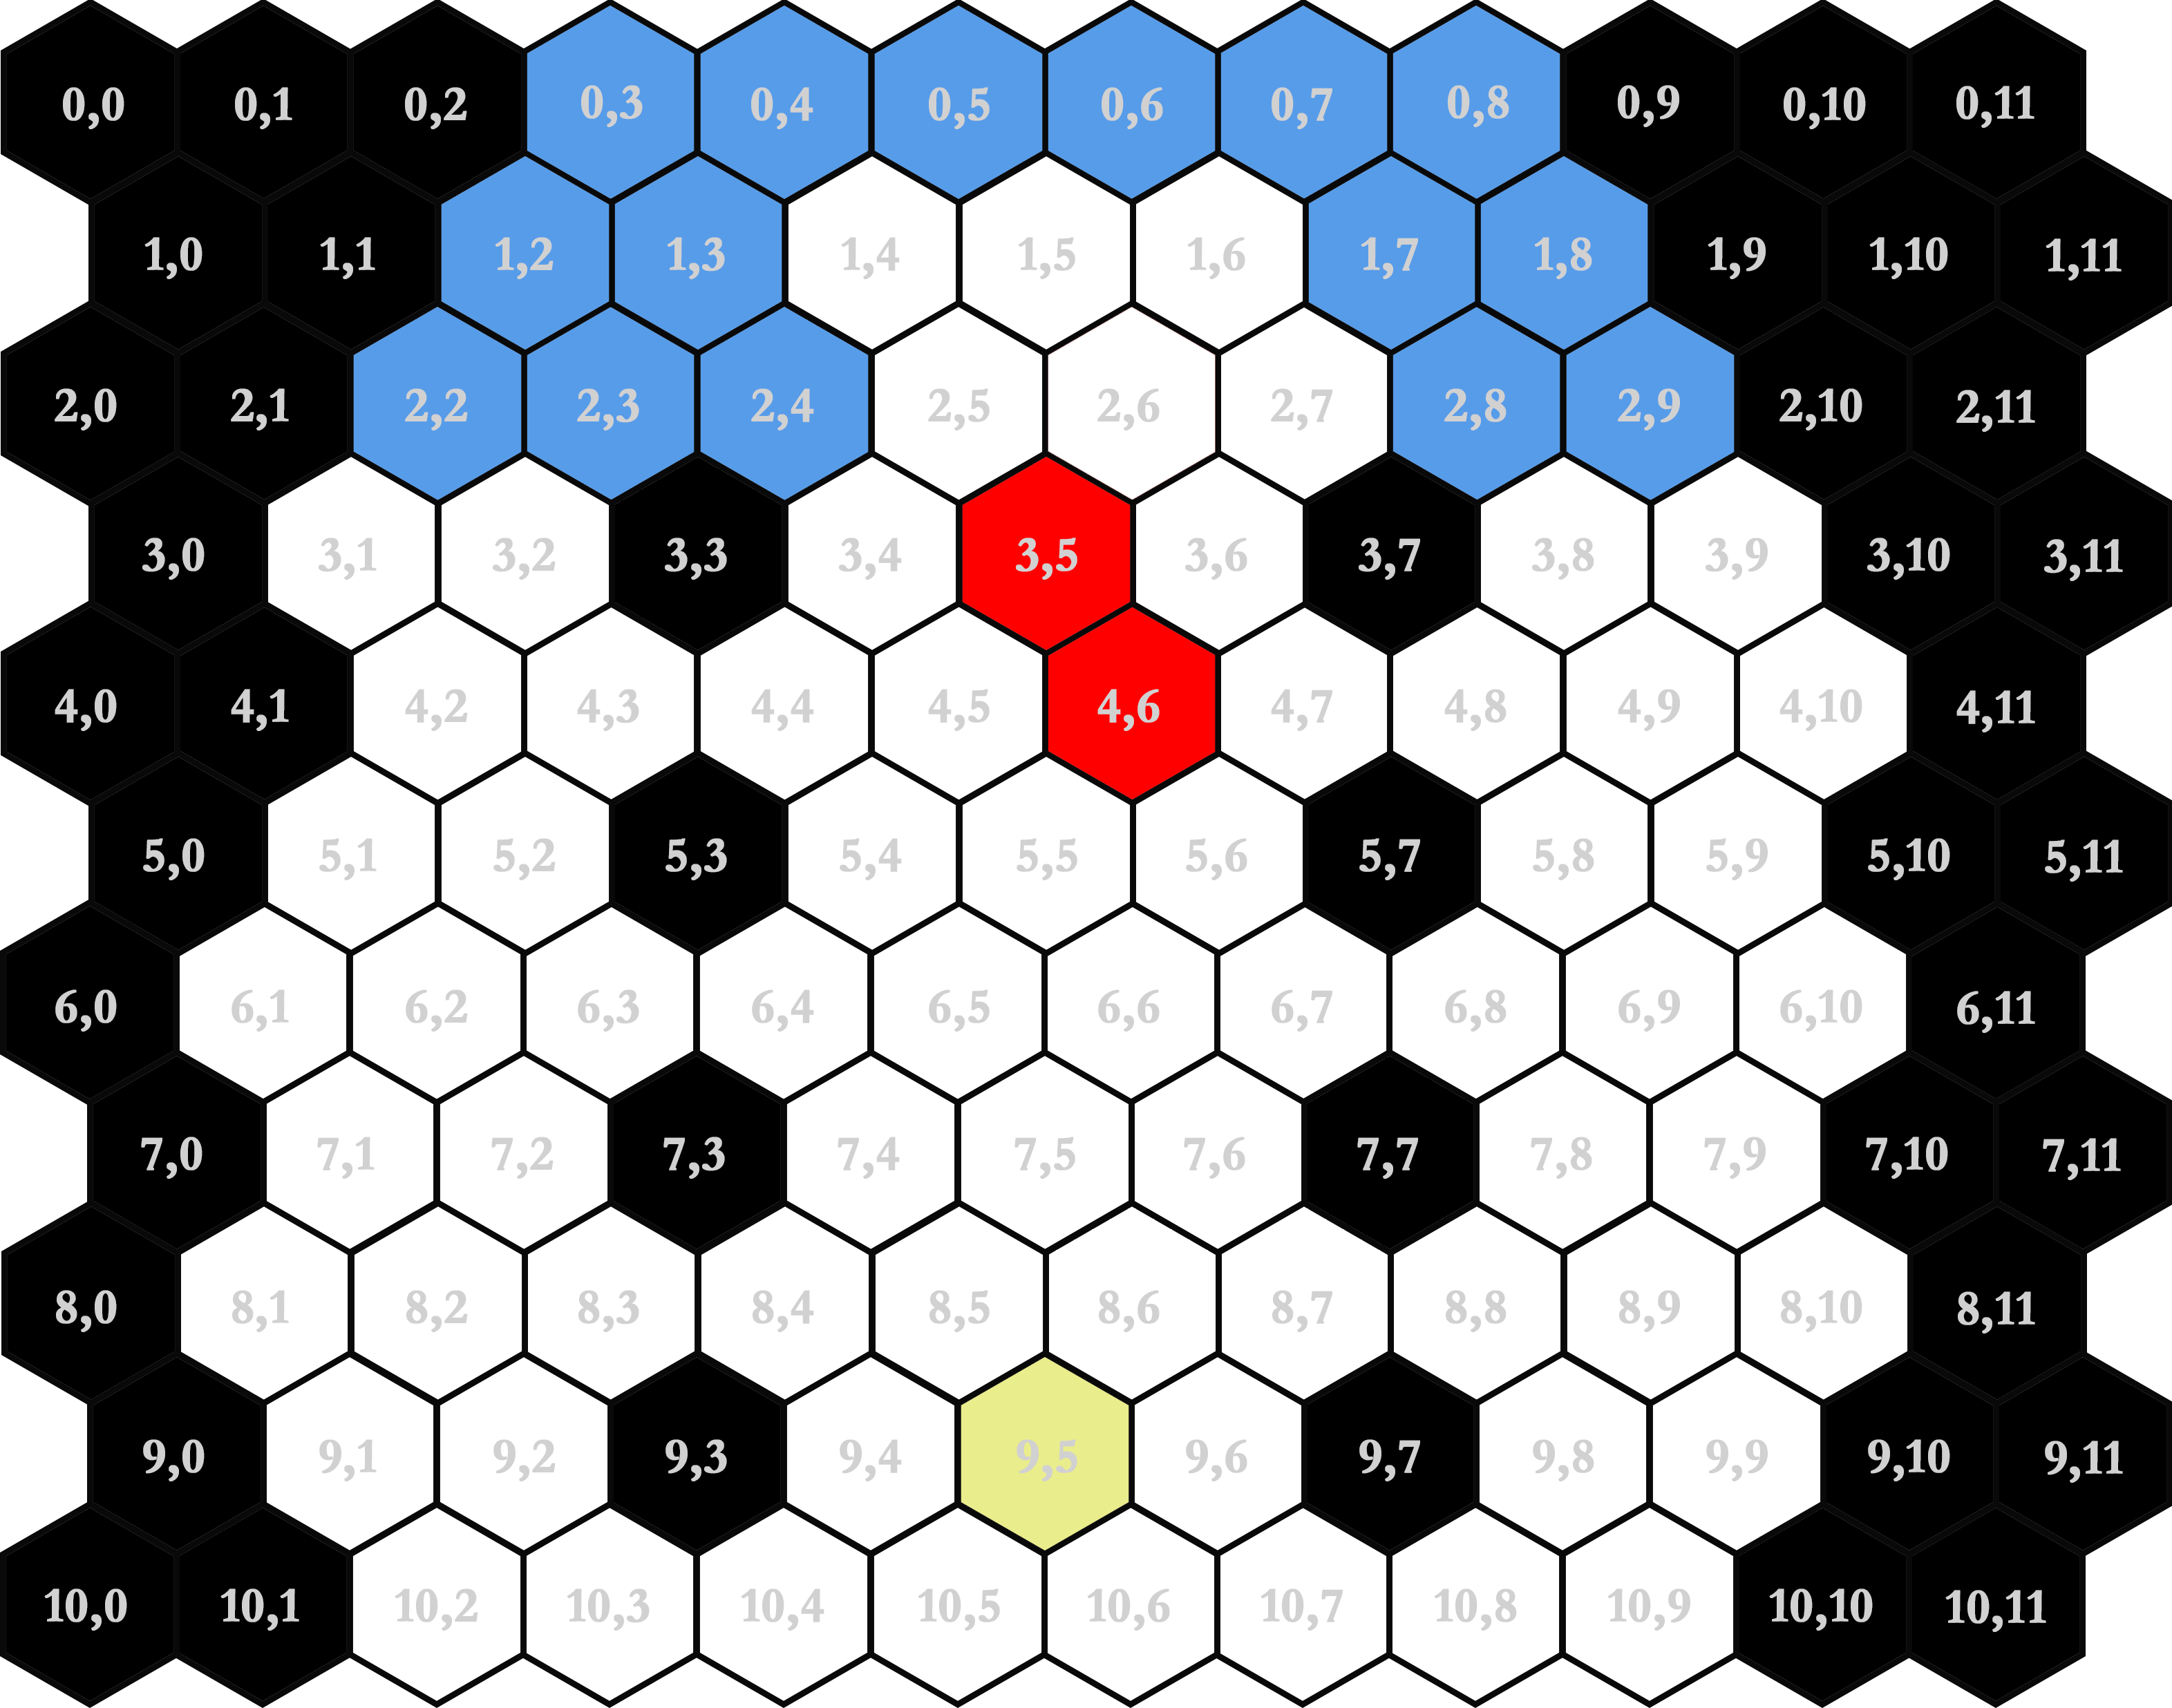
\includegraphics[width = 0.70\textwidth]{./maps/c320.png}
}
\end{center}

\subsection*{Setup Instructions}
\begin{itemize}
\item \textbf{Goldenrod:} Character Start Location. Place the character on either tile.
\item \textbf{Red:} Enemy Start Location. Place Snickersnee on these tiles.
\item \textbf{Black:} Impassable Boundary/Full-Cover
\end{itemize}

\pagebreak

\begin{tcolorbox}
\subsection*{Doom Events}
\begin{itemize}
\item \textbf{Round 4:} \emph{The beast roars and paws at the ground.} Snickersnee gains 1 Move value.
\item \textbf{Round 6:} \emph{The beast bristles and foams at the mouth.} Snickersnee gains 1 \textbf{P.DEF}.
\end{itemize}
\end{tcolorbox}

\subsection*{Assist Table}
Once per Round, the player may use a Free action to activate an assist. When activating an assist, cover that entry with a token. That entry is exhausted for the entire encounter, and may not be activated again. Some assists may only be activated if the player possesses their required note.
\begin{tcolorbox}
\begin{center}
\begin{tabular}{ L | L | L }
\multicolumn{1}{c|}{\textbf{Boon of Fire}} & 
\multicolumn{1}{c|}{\textbf{Boon of Magic}} & 
\multicolumn{1}{c}{\textbf{Furry Distraction}} \\
Add 1 Enhanced Weapon: Fire (1) condition token to the status sheet  &
Add 1 Enhanced Weapon: Magic (1) condition token to the status sheet &
\emph{Requires: c311a}\newline Inflict \emph{Inevitable} Knockdown on Snickersnee \\
\hline
\multicolumn{1}{c|}{\textbf{Secret Parable}} & 
\multicolumn{1}{c|}{\textbf{Unspoken Word}} \\
\emph{Requires: c317a}\newline Restore 2 \textbf{HP} slots on the status sheet and add 1 Enhanced Defense: \textbf{P.DEF} (1) condition token &
\emph{Requires: c325a}\newline \emph{Reaction.} The character may commit a Move 3 \emph{Dodge!} at no \textbf{SP} cost this turn, ignoring all \textbf{EQP} requirements\\
\end{tabular}
\end{center}
\end{tcolorbox}

\subsection*{Encounter Table}
\begin{tcolorbox}
\textbf{Roll:} 2D6
\begin{center}
\begin{tabular}{ L | L | L }
\multicolumn{1}{c|}{\textbf{2}} & 
\multicolumn{1}{c|}{\textbf{3}} & 
\multicolumn{1}{c}{\textbf{4-5}} \\
\emph{Sudden. Unearthly Roar} &
\textbf{A:} \emph{Hind Kick}\newline \textbf{B:} Move.  \emph{Pounce}&
\textbf{A:} \emph{Gore. Gore}\newline \textbf{B:} \emph{Charge} \\
\hline
\multicolumn{1}{c|}{\textbf{6}} & 
\multicolumn{1}{c|}{\textbf{7}} & 
\multicolumn{1}{c}{\textbf{8}} \\
\textbf{A:} \emph{Pounce}\newline \textbf{B:} Move. \emph{Gore} &
\textbf{A:} Sudden. \emph{Hind Kick}\newline \textbf{B:} Move. \emph{Gore. Gore} &
\textbf{A:} \emph{Pounce}\newline \textbf{B:} Move. \emph{Gore} \\
\hline
\multicolumn{1}{c|}{\textbf{9-10}} & 
\multicolumn{1}{c|}{\textbf{11}} & 
\multicolumn{1}{c}{\textbf{12}} \\
\textbf{A:} \emph{Gore. Gore}\newline \textbf{B:} \emph{Charge} &
\textbf{A:} \emph{Hind Kick}\newline \textbf{B:} Move.  \emph{Pounce} &
\emph{Sudden. Unearthly Roar} \\
\end{tabular}
\end{center}
\end{tcolorbox}

\subsection*{Enemy Sheets}
\hrule
\ \\
{\large \textbf{Snickersnee}}\\\\
\begin{tabular}{s s s}
\textbf{HP:} 22 & \textbf{Move:} 3\\
\textbf{P.DEF:} 1 & \textbf{F.DEF:} 2 & \textbf{M.DEF:} 1\\
\end{tabular}\\

\emph{Large:} This entity occupies two distinct tiles, and requires head and tail tokens.\\

\emph{Great Foe:} This entity ignores all conditions (such as Knockback and Knockdown) inflicted by normal sources, except Blazing and Bleeding, and is immune to Backstab (but not Coup de Grâce).\\

\emph{Tottering:} If this entity assigns 6 damage tokens to \textbf{HP} in a single Round, it is inflicted with Knockdown upon assigning the sixth token.\\

\textbf{Attacks:}
\begin{itemize}
\item \emph{Gore} -  Move 1. Deal 2 \emph{Unparryable} Pierce damage to an adjacent entity (from head tile).
\item \emph{Pounce} - Move 2. Deal 3 \emph{Unparryable} Crush damage and Knockdown in a half-moon pattern (from head tile).
\item \emph{Hind Kick} - Deal 3 Crush damage, Knockback 2, and Knockdown to an adjacent entity (from tail tile).
\item \emph{Charge} - Move 5 in a straight \& snaking line. Deal 3 Pierce damage, Knockback 3, and Knockdown to an adjacent entity (from head tile). If Snickersnee cannot land this attack, then Move 5 in a straight \& snaking line anyway.
\item \emph{Unearthly Roar} - Inflict \emph{Inevitable} Flinch on all hexes within 3 tiles (from head tile).
\end{itemize}

\pagebreak

\subsection*{Victory}
The beast is frantic in death: a wailing, panicked thing. Despite its monstrous appearances it is very much still a mortal animal. Great gushers of blood spill from its many wounds, and with one last cry it sinks down into a great pool of itself.\\

Vagabond Lor approaches, knife-in-hand, something that looks to have been pilfered from the kitchen. And, padding softly, he does the monster a great mercy.\\

>> \turnto{c41x1}

\subsection*{Defeat}
As your vision fades you can hear the Everloyal strike up a great panic. Their champion has fallen, and despite their zeal they cannot seem to place this event as part of His plan.\\
>> \turnto{c41x2}